\documentclass[11pt]{article}
%\renewcommand{\thesection}{\Roman{section}}  %zmiana section na rzymskie
\usepackage[utf8]{inputenc}
\usepackage[OT4]{polski}
\usepackage{tabularx}
\usepackage[margin=60pt]{geometry}
\usepackage{amsmath}
\usepackage{amsfonts}
\usepackage{listings} 
\usepackage[usenames,dvipsnames,table,xcdraw]{xcolor}
\usepackage{array}
\usepackage{sidecap} %do grafik
\usepackage{wrapfig} % j. w.
\usepackage{graphicx} %j.. w.
\usepackage{subfig} %j. w.
\usepackage{booktabs}
\usepackage{longtable}
\usepackage{hyperref}
\usepackage{multirow}



\title{Modelowanie trajektorii cząstek naładowanych w polu magnetycznym.}

\author{Paweł Rzońca}

\begin{document}

\maketitle

\section*{Wstęp}
Rozważmy ruch elektronu w obecności pola magnetycznego. Funkcja Lagrange'a ma w tym przypadku postać
\begin{equation}
	\mathcal{L} = \dfrac{m}{2}\dot{\vec{r}}\ ^2 +\dfrac{e}{2}\vec{r}\cdot (\dot{\vec{r}}\times\vec{B}).
\end{equation}

W cylindrycznym układzie współrzędnych z osią $z$ skierowaną równolegle do pola uzyskujemy następującą
funkcję Hamiltona
\begin{equation}
\mathcal{H}= \dfrac{1}{2m}\left( p_z^2+p_r^2+\dfrac{1}{r^2}p_{\varphi}^2\right)
	-\dfrac{eB}{2m}p_{\varphi}+\dfrac{e^2B^2}{8m}r^2\ .
\end{equation}
Z równań Hamiltona otrzymujemy następujące równania opisujące ruch elektronu:\\
$\dot{z}=\dfrac{p_z}{m}, \qquad \dot{p_z}=0,$\\
$\dot{\varphi}=\dfrac{p_{\varphi}}{mr^2}-\dfrac{eB}{2m} ,\qquad \dot{p_{\varphi}}=0,$\\
$\dot{r}=\dfrac{p_r}{m}, \qquad \dot{p_r} = \dfrac{p_{\varphi}^2}{mr^3}-\dfrac{e^2B^2r}{4m}.$\\

Energia całkowita układu jest równa funkcji Hamiltona
\begin{equation}
E=\mathcal{H}.
\end{equation}
\section*{Metodyka}
Ruch w kierunku równoległym do pola ($z$) separuje się od ruchu w kierunku prostopadłym do 
pola i jest ruchem jednostajnym. Rozwiązania numeryczne znajdziemy dla ruchu poprzecznego.
Równania rozwiązujemy iteracyjnie:\\
$\varphi_{i+1} = \varphi_i + \left( \dfrac{p_{\varphi ,i}}{mr_i^2}-\dfrac{eB}{2m}\right) \Delta t,$\\
$r_{i+1} = r_i+\dfrac{p_{r,i}}{m}\Delta t,$\\
$p_{\varphi,i+1} = const, $\\
$p_{r,i+1}=p_{r,i}+\left(\dfrac{p_{\varphi,i}^2}{mr_{i}^3}-\dfrac{e^2r_{i}B^2}{4m}\right)\Delta t.$\\
Dla uproszczenia rachunków numerycznych wszystkie parametry układu, tj $m,\ e$ i $B$ kładziemy równe jeden.
Pęd sprzężony ze wzpółrzędną $\varphi$ jest stały i jego również kładziemy równy jeden.
\section*{Wyniki}
W ćwiczeniu przyjęto następujące dane wejściowe:\\
$m=1$ kg,\\
$B=1$ T,\\
$e=1$ C, \\
$p_{\varphi,0}=1$ kg$\cdot$m$^2$/s,\\
$p_{z,0}=1$ kg$\cdot$m/s.\\
Rozpoczęto od wyboru kroku czasowego $\Delta t$. W tym celu zbadano wahania energii w czasie. Porównanie dla kilku 
wartości kroku czasowego przedstawiono na wykresie \ref{WE}. Do dalszej analizy 
wybrano krok $\Delta t=0,0001$ s, gdyż dla takiego kroku energia była w dobrym przybliżeniu stałą. 

\begin{figure}[h!]
\begin{center}
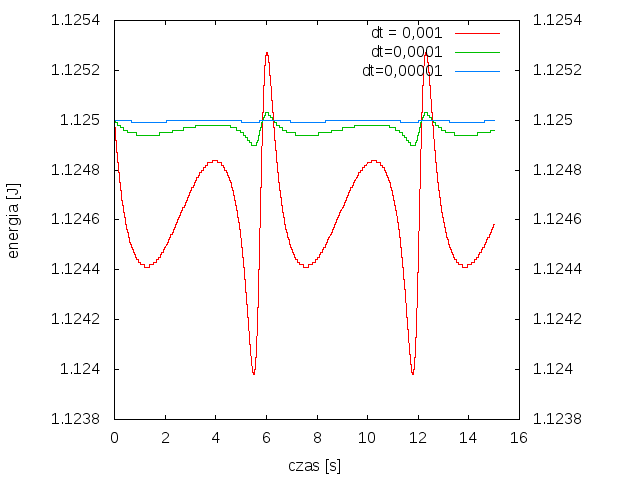
\includegraphics[width=0.6\textwidth]{en.png}
\caption{Zależność energii od czasy dla różnych kroków czasowych. Dane wejściowe: $r_0=1$ m,\\ 
		$p_{r,0}=1$ kg$\cdot$m/s, $\varphi_0=1$}{\label{WE}}
\end{center}
\end{figure}

Następnie wyznaczamy trajektorię dla różnych wartości początkowych $\varphi_0,\ r_0$ oraz $ p_{r,0}$.
Trajektorie ilustrujemy we współrzędnych kartezjańskich, na wykresach \ref{WF}, \ref{WR} oraz \ref{WP}.

\begin{figure}[h!]
\begin{center}
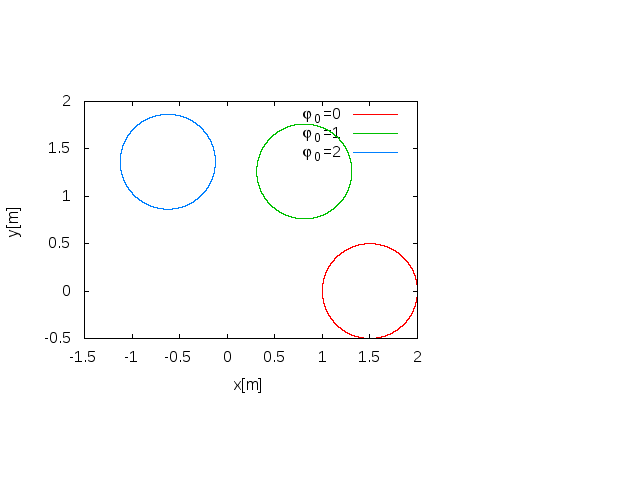
\includegraphics[width=0.7\textwidth]{fi.png}
\caption{Porównanie otrzymanych trajektorii dla różnych wartości początkowych $\varphi_0$. Pozostałe dane wejściowe:
		$r_0=1$ m, $p_{r,0}= 0$ kg$\cdot$m/s.}{\label{WF}}	
\end{center}
\end{figure}

\begin{figure}[h!]
\begin{center}
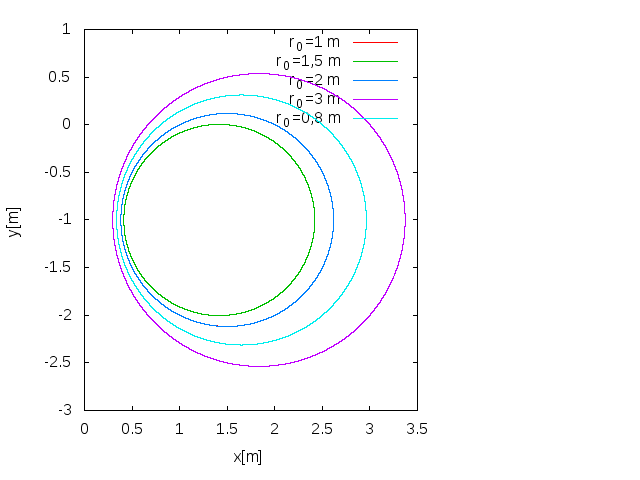
\includegraphics[width=0.7\textwidth]{pro2.png}
\caption{Porównanie otrzymanych trajektorii dla różnych wartości początkowych $r_0$. Pozostałe dane wejściowe:
		$\varphi_0=0$, $p_{r,0}= 1$ kg$\cdot$m/s.}{\label{WR}}	
\end{center}
\end{figure}

\begin{figure}[h!]
\begin{center}
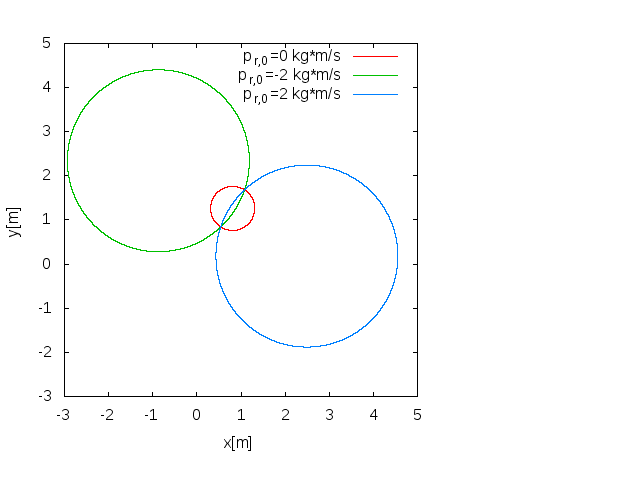
\includegraphics[width=0.7\textwidth]{ped.png}
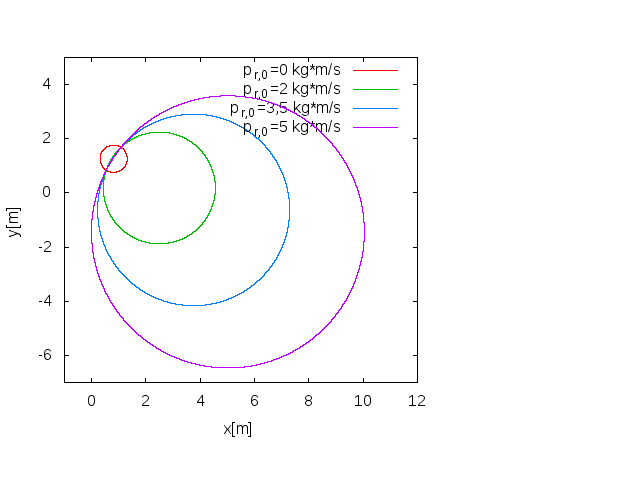
\includegraphics[width=0.7\textwidth]{ped2.png}
\caption{Porównanie otrzymanych trajektorii dla różnych wartości początkowych $p_{r,0}$. Pozostałe dane wejściowe:
		$r_0=1$ m, $\varphi= 1$. Trajektorii dla $r_0=1$ m nie widać na wykresie, gdyż pokrywa się ona z trajektorią dla $r_0=2$ m.}{\label{WP}}	
\end{center}
\end{figure}

\section*{Podsumowanie}
W każdym przypadku trajektoria (przy pominięciu ruchu wzdłuż osi $z$) pozostaje okręgiem. Zmiana $\varphi_0$ nie zmienia 
kształtu toru ruchu, a powoduje przesunięcie trajektorii o dany kąt, względem $\varphi_0=0$. Zmienna $\varphi$ nie występuje w rozważanych 
równaniach, prócz równania z którego je wyznaczamy, co powoduje niezależność kształtu trajektorii od jej początkowej wartości. Natomiat dla różnych $r_0$ 
otrzymujemy różne okręgi, bez prostej zależności (np. dla wartości $r_0=1$ m i $r_0=2$ m trajektorie pokrywają się). W przypadku $p_{r,0}$ okręgi po których 
porusza się ciało zwiększają średnicę wzraz ze wzrostem $p_{r,0}$.
\end{document}


